\section{Funcionalidades}
\label{funcionalidades}

%TODO explicar o formato de user stories e cenários de uso e correlacioanr
%com a seção que trata sobre desenvolvimento de software livre
%conceituar histórias de usuário, BDD, cenário de uso e teste de aceitação
%enfatizar que os requisitos não serão apresentados da maneira tradicional
%(mais próximo de como são definidos nas equipes ágeis e nas comunidades de
%software livre).

%TODO adicionar bibliografia sobre métodos ágeis e BDD.

As funcionalidades disponíveis no Noosfero, seja em seu \textit{core}
ou através de \textit{plugins}, nos permitiria fazer uso da plataforma como
um ambiente virtual para a troca de conhecimento através das comunidades e
perfis de usuários, e como portal para departamentos e organizações da
Universidade de Brasília. Entretanto, ainda com algumas lacunas, que avaliamos
como pertinentes de serem tratadas.
%
Nesta seção apresentamos as funcionalidades que julgamos mais interessantes
de implementarmos, dentro do prazo deste trabalho, para o Comunidade.UnB.
%
Dessa forma, descrevemos as funcionalidades desenvolvidas, que contaram com
nossa contribuição e que contribuíram para o crescimento do Comunidade.UnB.


Para melhor apresentarmos tais funcionalidades, o formato utilizado para
elaborar os requisitos foi o de Histórias de Usuários (\textit{User Stories}),
prática bastante difundida dentro das comunidades de métodos ágeis e também
adotada em algumas comunidades de software livre. 
%
Além das histórias, utilizamos também o formato de critérios de aceitação
apresentados por \citeonline{north2006}, outra
prática ágil que vem ganhando força com a popularização do BDD.
%
O formato adotado é conveniente para nós, uma vez que o Noosfero utiliza o
\textbf{cucumber}\footnote{\url{http://cukes.info/}}, uma ferramenta para
automatização de testes escritos em linguagem natural, criada para apoiar a
utilização de BDD. No \textbf{cucumber}, os testes são escritos no formato
de funcionalidades e cenários, utilizando os formatos de histórias de
usuário e de critérios de aceitação mencionados. A Figura
\ref{cucumber}~\footnote{Extraído de \url{https://github.com/cucumber/cucumber/wiki}}
apresenta um exemplo de uso do \textbf{cucumber}.

%TODO inserir código ao invés de imagem
\begin{figure}[h]
	\centering
	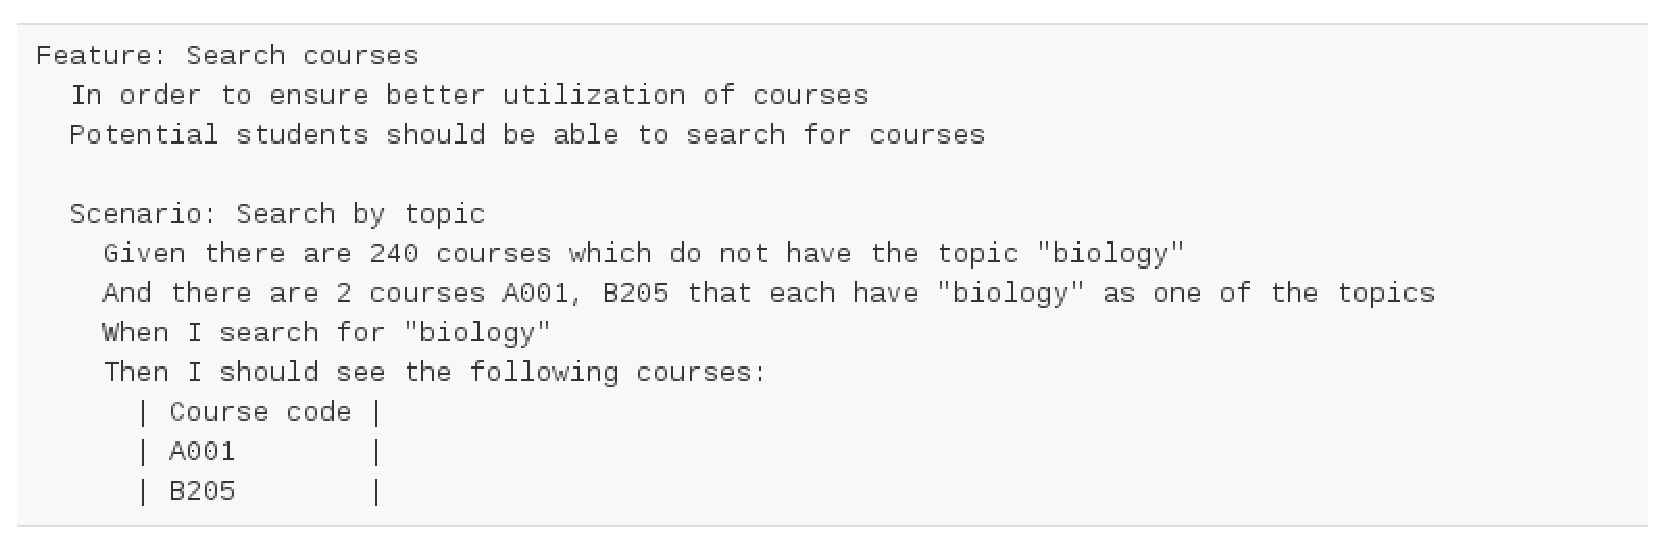
\includegraphics[keepaspectratio=true,scale=0.6]{figuras/cucumber_sample.eps}
	\caption{Exemplo de utilização do cucumber}
	\label{cucumber}
\end{figure}

Apesar do \textbf{cucumber} ter sido desenvolvido para que clientes e usuários,
não-técnicos, possam escrever as funcionalidades e os cenários em linguagem
próxima à linguagem natural, algumas regras devem ser seguidas uma vez que
a ferramenta precisa traduzir esses textos para uma linguagem que possa ser
interpretada por um computador, de forma a automatizar a execução dos testes.
%
Escrevemos os cenários descritos nesta seção, originalmente, em inglês no
\textit{issue tracker} do Noosfero e os traduzimos para o português,
o adaptando para um formato mais adequado para um texto científico.


%------------------------------funcionalidade---------------------------------%
\subsection{\textit{Plugin} Comunidade.UnB}

\subsubsection*{Histórias de usuário}

O \textit{plugin} Comunidade.UnB foi criado para suprir algumas necessidade de
integração de serviços fornecidos pela universidade e a rede de colaboração que
estamos implantando na UnB, como a autenticação via base de dados mantida pela universidade.
%
Assim, o usuário poderá ter acesso ao portal de comunidades através dos mesmos
dados utilizados para acessar outros serviços, como, por exemplo, o serviço de
matrícula para alunos ou o serviço de lançamento de notas para professores.

Ao ativar o \textit{plugin}, os campos utilizadas para realizar o \textit{login}
no sistema serão alterados para os mesmo campos utilizados em sistemas da
universidade, matrícula para alunos e prefixo do correio eletrônico para
professores e funcionários técnico-administrativos, e a senha será a mesma.

%TODO adicionar LDAP e CPD nas siglas
Portanto, o \textit{plugin} adiciona o campo matrícula e e-mail institucional
(caso o usuário deseje ter manter o campo de e-mail original para seu e-mail
pessoal), além de fazer a integração com o serviço de \textit{Lightweight
Directory Access Protocol} (LDAP)~\footnote{\url{%
http://en.wikipedia.org/wiki/Lightweight_Directory_Access_Protocol}}
no qual o CPD da UnB mantém os dados dos usuários. Contudo, o usuário, durante
seu primeiro \textit{login}, escolhe os campos nome de usuário, nome completo
e e-mail.

Foi necessário também retirar a funcionalidade de alteração de senha uma vez
que queremos manter a compatibilidade entre a rede Comunidade.UnB
e os demais serviços. Desta forma, caso o usuário deseje trocar sua senha, o
mesmo deve procurar o CPD e solicitar a alteração.

Até o momento da escrita deste texto, conseguimos autorização para utilizar
apenas a base de dados que contém os dados dos alunos, de forma que a
história de usuário e os cenários a seguir levarão em consideração apenas
a utilização do Comunidade.UnB pelos alunos, mas a funcionalidade
se mantém a mesma para professores e servidores técnico-administrativos que
queiram utilizar a rede.

%histórias
\begin{enumerate}

%--------------------------------história-------------------------------------%
\item \underline{Autenticação via LDAP da UnB}

\textbf{Como} um aluno da Universidade Brasília

\textbf{Eu quero} me autenticar na rede através da minha matrícula e senha
utilizada em outros sistemas.

\subsubsection*{Cenários de uso:}

%cenários
\begin{enumerate}

%---------------------------------cenário-------------------------------------%
\item \underline{Primeiro acesso}

\textbf{Dado} que sou aluno da UnB

\textbf{E} possuo cadastro ativo na base de dados da UnB

\textbf{E} nunca utilizei o serviço do Comunidade.UnB

\textbf{Quando} eu acessar o portal

\textbf{E} preencher os campos matrícula e senha com a matrícula e a senha
fornecidas a mim pela universidade

\textbf{Então} deverei ser direcionado para uma página com o título
"Primeiro Acesso"

\textbf{E} deverei ver os campos ``nome de usuário'', ``nome completo'' e
``e-mail pessoal'' em branco.

%---------------------------------cenário-------------------------------------%
\item \underline{Registro}

\textbf{Dado} que sou aluno da UnB

\textbf{E} me encontro na página de primeiro acesso do Comunidade.UnB

\textbf{Quando} eu preencher os campos
``nome de usuário'',\\
``nome completo''\\
e ``e-mail pessoal'' com ``daniel.bucher'',\\
``Daniel Costa Bucher'' e\\
``daniel.bucher88@gmail.com''

\textbf{E} clicar no botão ``Registrar''

\textbf{Então} eu devo ser direcionado para meu perfil

\textbf{E} devo ver a url ``<domínio>/daniel.bucher''

\textbf{E} devo ver ``Daniel Costa Bucher'' abaixo da imagem padrão de perfis
do Noosfero.

%---------------------------------cenário-------------------------------------%

\item \underline{Acesso}

\textbf{Dado} que sou aluno da UnB

\textbf{E} já utilizei o serviço do Comunidade.UnB

\textbf{Quando} eu entrar com minha matrícula e senha fornecida pela universidade
nos campos adequados para autenticação

\textbf{E} clicar em entrar

\textbf{Então} eu devo me encontrar \textit{logado} no sistema com a minha conta.

%cenários
\end{enumerate}

%histórias
\end{enumerate}

\subsubsection*{Desenvolvedores responsáveis:}

%desenvolvedores
\begin{enumerate}

\item Daniel Bucher - UnB

%desenvolvedores
\end{enumerate}

%------------------------------funcionalidade---------------------------------%
\subsection{Melhorias no \textit{plugin} de sub-organizações}
\label{feature:sub_organizations}

As histórias de usuários listadas nesta sub-seção dizem respeito a melhorias
no \textit{plugin} de sub-organizações do Noosfero e foram desenvolvidas em
conjunto com a Colivre e a equipe do Portal da Faculdade UnB Gama - FGA.

No Noosfero, uma organização é a abstração de uma entidade que pode assumir
o papel tanto de comunidade quanto de empreendimento. Os cenários de uso das
histórias a seguir foram especificados utilizando comunidades como exemplo,
mas as alterações realizadas afetam da mesma forma a relação entre usuários
e empreendimentos.

%TODO colocar figura da relação de heranças organização -> comunidade/empreendimento

O termo ``organização mãe'' é utilizado para designar uma organização que
possua sub-organizações, também chamadas de organizações filhas. Conforme
descrito acima, uma organização mãe pode ser tanto uma comunidade quanto um
empreendimento.

\subsubsection*{Histórias de usuário:}

%histórias de usuário
\begin{enumerate}

%--------------------------------história-------------------------------------%
\item \underline{Listar organizações `mãe' na lista de organizações de um usuário}

Esta história de usuário está mapeada no ActionItem de número 2825\footnote{\url
{https://noosfero.org/Development/ActionItem2825}}.

\textbf{Como} um usuário

\textbf{Eu quero} visualizar organizações mãe de sub-organizações que faço
parte junto à lista de minhas organizações.

\subsubsection*{Cenários de uso:}

%cenários
\begin{enumerate}

%---------------------------------cenário-------------------------------------%
\item \underline{Ver comunidade ``mãe'' na página ``Gerenciar meus grupos''}

\textbf{Dado} que eu estou logado com a usuário ``ze''

\textbf{E} ``ze'' não é membro do Comunidade.UnB

\textbf{E} ``ze'' é membro da sub-comunidade de Unb, FGA

\textbf{Quando} eu navegar até a página ``Gerenciar meus grupos''
(/myprofile/ze/memberships)

\textbf{Então} eu tenho que ver o Comunidade.UnB listada junto às
demais comunidades que faço parte.

%---------------------------------cenário-------------------------------------%
\item \underline{Ver comunidade ``mãe'' na página ``Comunidades de ze''}

\textbf{Dado} que eu estou logado com a usuário ``ze''

\textbf{E} ``ze'' não é membro do Comunidade.UnB

\textbf{E} ``ze'' é membro da sub-comunidade de Unb, FGA

\textbf{Quando} eu navegar até a página ``Comunidades de ze''
(/profile/ze/communities)

\textbf{Então} eu tenho que ver o Comunidade.UnB listada junto às
demais comunidades que faço parte.

%cenários
\end{enumerate}

%--------------------------------história-------------------------------------%
\item \underline{Bloco de organizações relacionadas}

Esta história de usuário está mapeada no \textit{issue} de número 2499\footnote{\url
{https://noosfero.org/Development/ActionItem2499}}.

\textbf{Para} ter acesso às organizações relacionadas a uma organização

\textbf{Como} um usuário

\textbf{Eu quero} visualizar um bloco que liste todas as organizações
relacionadas à organização atual.

\subsubsection*{Cenários de uso:}

%cenários
\begin{enumerate}

%---------------------------------cenário-------------------------------------%
\item \underline{Adicionar um bloco de sub-organizações}

\textbf{Dado} que eu estou logado com meu usuário

\textbf{E} meu usuário é administrador da comunidade X

\textbf{Quando} eu navegar até o painel de controle da comunidade X

\textbf{E} eu clicar em ``Editar blocos laterais''

\textbf{E} eu clicar em ``Adicionar bloco''

\textbf{Então} eu tenho que ver a opção ``Organizações Relacionadas''.

%---------------------------------cenário-------------------------------------%
\item \underline{Listar todas as sub-organizações na organização ``mãe''}

\textbf{Dado} que eu estou logado com meu usuário

\textbf{E} meu usuário é membro da comunidade X

\textbf{E} e a comunidade Y é uma sub-comunidade de X

\textbf{E} e o empreendimento Z é um sub-empreendimento de X

\textbf{E} a comunidade X possua um bloco de organizações relacionadas

\textbf{Quando} eu navegar até a página da comunidade X

\textbf{Então} eu tenho que ver um bloco com o título ``Sub organizações''.

\textbf{E} eu tenho que ver um \textit{link} para a sub-comunidade Y neste
bloco

\textbf{E} eu tenho que ver um \textit{link} para o sub-empreendimento Z neste
bloco.

%---------------------------------cenário-------------------------------------%
\item \underline{Listar apenas as sub-comunidades organização `mãe'}

\textbf{Dado} que eu estou logado com meu usuário

\textbf{E} meu usuário é membro da comunidade X

\textbf{E} e a comunidade Y é uma sub-comunidade de X

\textbf{E} e o empreendimento Z é um sub-empreendimento de X

\textbf{E} a comunidade X possua um bloco de organizações relacionadas

\textbf{E} o bloco esteja configurado para mostrar apenas comunidades

\textbf{Quando} eu navegar até a página da comunidade X

\textbf{Então} eu tenho que ver um bloco com o título ``Sub-comunidades''.

\textbf{E} eu tenho que ver um \textit{link} para a sub-comunidade Y neste
bloco

\textbf{E} eu não tenho que ver um \textit{link} para o sub-empreendimento Z
neste bloco.

%---------------------------------cenário-------------------------------------%
\item \underline{Visualizar página de sub-organizações de uma organização `mãe'}

\textbf{Dado} que eu estou logado com meu usuário

\textbf{E} meu usuário é membro da comunidade X

\textbf{E} e a comunidade Y é uma sub-comunidade de X

\textbf{E} e o empreendimento Z é um sub-empreendimento de X

\textbf{E} a comunidade X possua um bloco de organizações relacionadas

\textbf{Quando} eu navegar até a página da comunidade X

\textbf{E} eu clicar no link ``Ver todos'' do bloco de organizações relacionadas

\textbf{Então} eu tenho que ver uma página de sub-organizações

\textbf{E} eu tenho que ver um \textit{link} para a sub-comunidade Y neste
bloco

\textbf{E} eu tenho que ver um \textit{link} para o sub-empreendimento Z
neste bloco.

%---------------------------------cenário-------------------------------------%
\item \underline{Visualizar página de sub-comunidades de uma organização `mãe'}

\textbf{Dado} que eu estou logado com meu usuário

\textbf{E} meu usuário é membro da comunidade X

\textbf{E} e a comunidade Y é uma sub-comunidade de X

\textbf{E} e o empreendimento Z é um sub-empreendimento de X

\textbf{E} a comunidade X possua um bloco de organizações relacionadas

\textbf{E} o bloco esteja configurado para mostrar apenas comunidades

\textbf{Quando} eu navegar até a página da comunidade X

\textbf{E} eu clicar no link ``Ver todos'' do bloco de organizações relacionadas

\textbf{Então} eu tenho que ver uma página de sub-organizações

\textbf{E} eu tenho que ver um \textit{link} para a sub-comunidade Y neste
bloco

\textbf{E} eu não tenho que ver um \textit{link} para o sub-empreendimento Z
neste bloco.

%---------------------------------cenário-------------------------------------%
\item \underline{Listar todas as organizações ``mãe'' de uma organização}

\textbf{Dado} que eu estou logado com meu usuário

\textbf{E} meu usuário é membro da comunidade X

\textbf{E} e a comunidade Y é ``mãe'' de X

\textbf{E} e o empreendimento é ``pai'' de X

\textbf{E} a comunidade X possua um bloco de organizações relacionadas

\textbf{Quando} eu navegar até a página da comunidade X

\textbf{Então} eu tenho que ver um bloco com o título ``Organizações pais''.

\textbf{E} eu tenho que ver um \textit{link} para a sub-comunidade Y neste
bloco

\textbf{E} eu tenho que ver um \textit{link} para o sub-empreendimento Z neste
bloco.

%cenários
\end{enumerate}

%--------------------------------história-------------------------------------%
\item \underline{Visualização completa nas páginas de organização relacionadas}

\textbf{Como} um usuário

\textbf{Eu quero} visualizar informações sobre as organizações relacionadas nas
páginas de organizações relacionadas

\textbf{Para} me informar sobre elas sem precisar visitar a página de cada uma.

\subsubsection*{Cenários de uso:}

%cenários
\begin{enumerate}

%---------------------------------cenário-------------------------------------%
\item \underline{Visualizar modo completo na página de sub-organizações}

\textbf{Dado} a comunidade X

\textbf{E} a comunidade Y é `filha' de X

\textbf{E} o empreendimento Z é `filho' de X

\textbf{Quando} eu navegar até a página de sub-organizações de X

\textbf{E} eu clicar na opção de visualização completa

\textbf{Então} eu tenho que ver as informações

%cenários
\end{enumerate}

%histórias de usuário
\end{enumerate}

%-----------------------------------------------------------------------------%

\subsubsection*{Desenvolvedores responsáveis:}

Os seguintes colaboradores do Noosfero participaram do desenvolvimento desta
funcionalidade:

%desenvolvedores
\begin{enumerate}

\item Aurélio A. Heckert - Colivre

\item Daniel Bucher - UnB

\item Equipe do Portal FGA - UnB

%desenvolvedores
\end{enumerate}

%------------------------------funcionalidade---------------------------------%
\subsection{\textit{Plugin} de bloco de video}

Esta funcionalidade foi desenvolvido pela equipe do Portal
da FGA e está mapeada no \textit{issue} de número 2823\footnote{\url{https://
noosfero.org/Development/ActionItem2823}} e consiste em um \textit{plugin}
que adicionar um novo tipo de bloco no Noosfero, o VideoBlock.

Este bloco incorpora vídeos de plataformas externas, atualmente o Vimeo
e o Youtube, dentro de seu conteúdo.

%histórias
\begin{enumerate}

%--------------------------------história-------------------------------------%
\item \underline{Bloco de video}

\textbf{Para} adicionar vídeos em um perfil do Noosfero

\textbf{Como} um usuário

\textbf{Eu quero} ter um bloco em que eu possa adicionar um vídeo de plataformas
como o Youtube\footnote{\url{https://youtube.com}} e o Vimeo\footnote{\url{https://
vimeo.com}}.

\subsubsection*{Cenários de uso:}

%cenários
\begin{enumerate}

%---------------------------------cenário-------------------------------------%
\item \underline{Adicionar bloco}

\textbf{Dado} que estou logado como o usuário ``Zé''

\textbf{E} o \textit{plugin} Video esteja atualizado

\textbf{Quando} eu navegar até a página ``Editar blocos laterais'' do meu perfil

\textbf{E} clicar em ``Adicionar bloco''

\textbf{E} selecionar ``Bloco de vídeo''

\textbf{E} clicar em ``Adicionar''

\textbf{Então} eu devo ver um bloco de vídeo sem conteúdo na área principal.


%---------------------------------cenário-------------------------------------%
\item \underline{Adicionar vídeo do Youtube}

\textbf{Dado} que estou logado como o usuário ``Zé''

\textbf{E} possui um bloco de vídeo no meu perfil

\textbf{Quando} eu navegar até a página de ``Editar blocos laterais'' do meu perfil

\textbf{E} clicar em ``Editar'' no bloco de vídeo

\textbf{E} adicionar a URL de um video do Youtube

\textbf{E} preencher os campos ``Largura'' e ``Altura'' com 536 e 360
respectivamente

\textbf{E} clicar em ``Salvar''

\textbf{Então} eu devo ver o vídeo incorporado na área principal do meu
perfil na resolução ``536x360''.


%---------------------------------cenário-------------------------------------%

\item \underline{Adicionar vídeo do Vimeo}

\textbf{Dado} que estou logado como o usuário ``Zé''

\textbf{E} possui um bloco de vídeo no meu perfil

\textbf{Quando} eu navegar até a página de ``Editar blocos laterais'' do meu perfil

\textbf{E} clicar em ``Editar'' no bloco de vídeo

\textbf{E} adicionar a URL de um video do Vimeo

\textbf{E} preencher os campos ``Largura'' e ``Altura'' com 536 e 360
respectivamente

\textbf{E} clicar em ``Salvar''

\textbf{Então} eu devo ver o vídeo incorporado na área principal do meu
perfil na resolução ``536x360''.

%cenários
\end{enumerate}

%histórias
\end{enumerate}

\subsubsection*{Desenvolvedores responsáveis}

Os seguintes colaboradores do Noosfero participaram do desenvolvimento desta
funcionalidade:

%desenvolvedores
\begin{enumerate}

\item Daniel Bucher - UnB

\item Equipe do Portal FGA - UnB

%desenvolvedores
\end{enumerate}


\begin{comment}
 
%TODO revisar funcionalidade
%------------------------------funcionalidade---------------------------------%
\subsection{Usabilidade do bloco \textit{links}}

%TODO Dividir em mais de uma user story

Implementar melhorias no Bloco ``Links'', para que fique muito mais intuitivo
para um usuário personalizar o seu menu lateral. Incluindo;
- Mover itens por meio de ``Drag and Drop''
- Interface fácil de incluir links para conteúdo próprio.

Implementar melhorias no bloco ``links'' para aumentar a usabilidade:
  - Permitir reorganização de link via ``drag and drop''
  - Interface fácil de inserir links para conteúdo

\subsubsection*{Histórias de usuário}

\begin{enumerate}


%--------------------------------história-------------------------------------%
\item \underline{Mover itens por \textit{Drag and Drop}}

\textbf{Como} um usuário do Noosfero

\textbf{Eu quero} reordenar os items de um bloco de \textit{links} por meio de
\textit{Drag and Drop}.

\subsubsection*{Cenários de uso}

\begin{enumerate}

\item \underline{Arrastar um item}

\textbf{Dado} que eu estou logado com meu usuário

\textbf{E} estou na página de edição de blocos laterais

\textbf{E} eu clico no botão de edição do bloco padrão de links

\textbf{E} eu veja ``Perfil'' em cima de ``Galeria de imagens''

\textbf{Quando} arrastar ``Galeria de imagens'' para cima de ``Perfil''

\textbf{E} clicar no botão ``Salvar''

\textbf{E} eu for para a página do meu perfil

\textbf{Então} eu tenho que ver ``Galeria de imagens'' em cima de ``Perfil''
no bloco de links padrão do perfil.

\end{enumerate}

%--------------------------------história-------------------------------------%
\item \underline{\textit{Auto-complete} ao adicionar novos itens}
%TODO elaborar user story

\end{enumerate}

\end{comment}

